\documentclass[
  11pt,					% Schriftgröße
  DIV=13,				% Seitenlayout (Satzspiegel)
  parskip=quarter,		% Abstand zwischen Absätzen
  oneside,				% Einseitig
%  headsepline,
  headings,	
%  draft,				% Korrekturfassung
  ]{scrreprt}			% scrartcl	

\usepackage{tikz,pgfplots}
\usepackage[utf8]{inputenc}
\usepackage[ngerman,english]{babel}
\selectlanguage{english}

\usepackage{graphicx}
\usepackage{float}
\graphicspath{{bilder/}}
\usepackage{svg}
\usepackage{listings}
\usepackage{verbatim}
\usepackage{lmodern}
\definecolor{codegreen}{rgb}{0,0.6,0}
\definecolor{codegray}{rgb}{0.5,0.5,0.5}
\definecolor{codepurple}{rgb}{0.58,0,0.82}
\definecolor{backcolour}{rgb}{0.95,0.95,0.92}


\lstdefinestyle{mystyle}{
	backgroundcolor=\color{backcolour},   
	commentstyle=\color{codegreen},
	keywordstyle=\color{magenta},
	numberstyle=\tiny\color{codegray},
	stringstyle=\color{codepurple},
	basicstyle=\ttfamily\footnotesize,
	breakatwhitespace=false,         
	breaklines=true,                 
	captionpos=b,                    
	keepspaces=true,                 
	numbers=left,                    
	numbersep=5pt,                  
	showspaces=false,                
	showstringspaces=false,
	showtabs=false,                  
	tabsize=2
}
\lstset{style=mystyle}


% Blindtext
\usepackage{blindtext}
 
% Schrifteinstellungen
\usepackage{lmodern} 		% Vektorschrift
\renewcommand{\familydefault}{\sfdefault}
\usepackage{sansmath}
\sansmath 
\usepackage{microtype}
\usepackage{acronym}
% Literatur einbinden
\usepackage{csquotes}	% Steuerung der Anführungszeichen
\usepackage[
  sorting=none,
  backend=biber,		% Sortier-Compiler
  style=numeric-comp,	% Zitationsstil
  ]{biblatex}

% Mathemodus
\usepackage{amsmath,amssymb}

% Trennung
\hyphenation{Crash-zo-ne}                    
\addbibresource{quellen.bib} %Citavi Reference Datei

% Kopf- und Fußzeile
\usepackage[
headsepline,	% Kopfzeilen-Sepparationslinie
automark,		% Lebende Kolumnentitel
]
{scrlayer-scrpage}
\pagestyle{scrheadings}		

\ohead*{\headmark}

\usepackage{abstract}
\usepackage{adjustbox}
\usepackage{tabularx}
\usepackage[T1]{fontenc}
%%%%%%%%%%%%%%%%%%%%%%%%%%%%%%%%%%%%%%%%%%%%%%%%%
%%%%%%%%%%%%%%%%%%%%%%%%%%%%%%%%%%%%%%%%%%%%%%%%%
%%%%%%%%%%%%%%%%%%%%%%%%%%%%%%%%%%%%%%%%%%%%%%%%%
%%%%%%%%%%%%%%%%%%%%%%%%%%%%%%%%%%%%%%%%%%%%%%%%%
%%%%%%%%%%%%%%%%%%%%%%%%%%%%%%%%%%%%%%%%%%%%%%%%%
%%%%%%%%%%%%%%%%%%%%%%%%%%%%%%%%%%%%%%%%%%%%%%%%%
%%%%%%%%%%%%%%%%%%%%%%%%%%%%%%%%%%%%%%%%%%%%%%%%%
%%%%%%%%%%%%%%%%%%%%%%%%%%%%%%%%%%%%%%%%%%%%%%%%%



% Titelseite
\titlehead{
  \begin{center}
  	\includegraphics[width=0.5\textwidth]{thi_logo_cropped}
  \end{center}
}

\title{Development of a mobile application for the algorithmic attribution of symptoms to potential diseases}

\subtitle{ \vspace{2ex} \LARGE BACHELOR THESIS}

\author{Angelina Petzold\\Immatriculation Number: 00108359}

\date{}

\publishers{
  \begin{tabular}{rl}
   \textbf{First Examiner} 		& Prof. Dr. Sebastian Apel 	\\
   \textbf{Second Examiner} 	& Prof. Dr. Marc Aubreville \\
   \textbf{Start Date} 			& October 11, 2022 		\\
   \textbf{Submission Date} 	& March 11, 2023		\\
  \end{tabular}
  }
  
% Rückseite der Titelseite
\uppertitleback{\begin{center}
		Development of a mobile application for the algorithmic attribution of symptoms to potential diseases
\end{center}}

\lowertitleback{\begin{center}
Technische Hochschule Ingolstadt
	\end{center}}



\newcommand\frontmatter{%
	\cleardoublepage
	%\@mainmatterfalse
	\pagenumbering{roman}}

\newcommand\mainmatter{%
	\cleardoublepage
	% \@mainmattertrue
	\pagenumbering{arabic}}

\begin{document}

  \maketitle
  
  \frontmatter
  
  
%% ABSTRACT %%

\selectlanguage{english}
{
	\raggedbottom
	\centering
	\vspace{0.9cm}
	\large
	\textbf{ABSTRACT}
	
	\adjustbox{minipage=0.8\textwidth}{
		\vspace{1.5cm} 
		  
	\par}
 	\pagebreak

	\selectlanguage{ngerman}
	\vspace{0.9cm}
	\large
	\textbf{PREAMBLE}
	
	\adjustbox{minipage=0.8\textwidth}{
		\vspace{1.5cm} 
		   
	\par}
	\pagebreak

	\selectlanguage{ngerman}
	\vspace{0.9cm}
	\large
	
	\textbf{\centering ACKNOWLEDGEMENTS}
	\vspace*{\fill}

	Mein hauptsächlicher Dank gilt meinem Betreuer Professor Doktor Sebastion Apel für seine hilfreichen Anregungen während des gesamten Betreuungszeitraumes. Die Freiheit, die er mir bei der Wahl des Themas gelassen hat, war nicht selbstverständlich.
	\newline \\
	Auch die Teilnehmerinnen und Teilnehmer meiner Befragung haben durch ihre Auskunftbereitschaft und interessanten Beiträge meine Bachelorarbeit wesentlich mitgeprägt.
	\newline \\
	Letztlich richte ich auch ein Dankeschön an meine Kommilitonin  Frau Jenny Hofbauer für das ausführliche Korrekturlesen und dem Mut machen während der gesamten Arbeit.
	
	\vspace{1cm}
	\noindent\hfil\rule{0.5\textwidth}{.4pt}\hfil
	\vspace{1cm}
	
	My main thanks go to my supervisor Professor Doctor Sebastion Apel for his helpful suggestions during the whole period of supervision. The freedom he gave me in choosing the topic was not self-evident.
	\newline \\
	The participants in my survey also played a major role in shaping my bachelor thesis through their willingness to provide information and interesting contributions.
	\newline \\
	Finally, I would also like to thank my fellow student Ms. Jenny Hofbauer for her detailed proofreading and encouragement throughout the thesis.
	\vspace*{\fill}
	\pagebreak


\par}
  
  \tableofcontents
  \chapter*{Acronyms}
  \addcontentsline{toc}{chapter}{Acronyms}
  
  \begin{acronym}
  	\acro{BÄK}{Bundesärztekammer; German Medical Association}
  	\acro{AI}{Artifical Intelligence}
  	\acro{API}{Application Programming Interface}
  	\acro{SDK}{Software Development Kit}
  	\acro{OOP}{Object Orientated Programming}
  	\acro{SRP}{Single Responsibility Principle}
  	\acro{OCP}{Open-Closed Principle}
  	\acro{LSP}{Liskov Substitution Principle}
  	\acro{ISP}{Interface Segregation Principle}
  	\acro{DIP}{Dependeny Inversion Principle}
  	\acro{BaaS}{Backend as a Service}
  	\acro{BÄK}{Bundesärztekammer; German Medical Association}
  	\acro{AI}{Artifical Intelligence}
  	\acro{API}{Application Programming Interface}
  	\acro{SDK}{Software Development Kit}
  	\acro{OOP}{Object Orientated Programming}
  	\acro{SRP}{Single Responsibility Principle}
  	\acro{OCP}{Open-Closed Principle}
  	\acro{LSP}{Liskov Substitution Principle}
  	\acro{ISP}{Interface Segregation Principle}
  	\acro{DIP}{Dependeny Inversion Principle}
  	\acro{BaaS}{Backend as a Service}
  \end{acronym}
  \mainmatter
  
  
%% INTRODUCTION %% 

\chapter{Introduction}
The current problem is described in the introduction, from which the motivation behind the bachelor thesis emerges. Subsequently, the goals that are pursued with the work are described.

\section{The Bachelor's Thesis Problem}
People in Germany are becoming more interested in physical and mental health matters. This is most likely attributed to the COVID-19 pandemic that has been circulating in recent years. \cite{.bahn-bonn} Along with positive outcomes, such as increased care for fellow citizens \cite{.bahn-bonn} and greater awareness of health issues, the consistent growth of interest in health issues also is causing problems. With an increasing number of anxious and concerned patients, medical practices and general practitioners have long since exceeded their capacity limits and have reached their breaking point \cite{.sok}. Patients also notice this: Overcrowded waiting rooms, long waiting periods, and nerve-racking telephone loops are becoming the norm for doctor visits. The BÄK (Bundesärztekammer), German Medical Association, draws attention to a second issue: as society ages, so does the medical industry. Every fifth doctor is about to retire. More than 13\% of doctors are between the ages of 60 and 65, while another 8.5\% are over the age of 65. Over the following few years, this will exacerbate clinics' and offices' already stressful staffing situation \cite{.blatt}. 
The bachelor`s thesis problem can be traced back to the preceding situation. The population is fearful, mainly caused by the COVID-19 pandemic, and doctors are reaching their limits. The resulting problems are of great importance. General practitioners are forced to order patient stops and issue access bans \cite{.sok}. This also means that patients needing immediate medical attention may be turned away, and medical care may be denied. In addition to the concerned patients, the number of seriously (COVID-19) ill people has steadily increased. There have been approximately 146,000 deaths in Germany since the start of the pandemic (as of August 19, 2022). \cite{.rki} As part of this work, a survey was launched to highlight the problem in more detail. The results indicate that around 80\% of those questioned have put off a visit to the doctor in recent years, even though they have suffered from symptoms.
\begin{figure}[H]
	\centering
	\includegraphics[scale=0.3]{avoidingDoctorYesNo.png}
	\caption[Survey Question]{Survey Question - Avoiding to visit the doctor}
\end{figure}
\noindent 
Another question in this survey asked respondents to list the justifications for delaying these doctor visits or the reasons they might consider forgoing a visit to the doctor. Those reasons range from long waiting times to difficulties scheduling an appointment. Figure 1.2 shows the mentioned distribution of the answers.
\begin{figure}[H]
	\centering
	\includegraphics[scale=0.4]{reasonsPuttingOf.png}
	\caption[Survey Question]{Survey Question - Reasons of avoiding to visit the doctor}
\end{figure}
\noindent 
All questions of the survey, together with the answers, can be found in appendix A.
\section{Motivation}
The mentioned problem imposes the question of addressing patients’ concerns while relieving the burden on doctors. Digitalization provides a solution to this problem. Online consultation hours and appointment scheduling have recently helped relieve medical practices. Smartphones, in particular, are becoming an increasingly important part of our daily lives. The goal of this bachelor thesis is to provide a method for efficiently minimizing the problems mentioned above through the use of mobile applications. Such an application can advise a worried user and help alleviate their fears.

\section{The Bachelor Thesis Goal}
The goals of the bachelor thesis can be defined as follows:
\begin{itemize}
	\item Requirements analysis for the application
	\item Design and conception of the application
	\item Creation of a firestore database
	\item Comparing different algorithmic disease assignment methods
\end{itemize}
The application should be able to generate a diagnosis based on a user's specified symptoms. This diagnosis is made after successful data gathering regarding the user's symptoms and a subsequent determination of the possible diseases. Another goal of the application is that doctors can expand the database, whereby a verification possibility must be provided to ensure that the person trying to log in is, in fact, a doctor. They should be provided with the possibility to add disease-related data or advice regarding diseases and illnesses for users. In general, this is to create a place for users to get information regarding their health status and, at the same time, get advice on how to improve it.

\chapter{Related Works}
This chapter provides an overview of a selection of mobile applications comparable to the one in this work.

\section{Mobile Applications}
\subsubsection{ADA} 
\textbf{ADA} is the most prevalent symptom-detection smartphone application. According to their statements, their users are currently around 12 million, while 28 million symptom analyses have already been completed \cite{.adaHOME}. The application is free in the PlayStore and the Apple Store. Disease detection in the ADA application is based on AI (Artificial Intelligence) developed by medical professionals of the ADA team. The user can provide personal data in their user profile, such as allergies and medication intake. A symptom analysis starts by asking the user what their worst symptom is. Based on the user's answer, the AI searches its medical lexicon for this symptom and asks a symptom-specific question.
An example of this would be to ask the user if he had enough water today for the symptom headache. ADA uses a specially developed reasoning technology to assign symptoms. For this purpose, each symptom and each disease was assigned a joint probability, which makes it possible to calculate the overall probability of the disease for the specific symptom analysis \cite{.adaKI}. After the successful diagnosis, the user can download the diagnosis in PDF format, while they are also saved internally. The ADA application also makes its collection of knowledge available to users in the form of a disease dictionary. ADA also offers an API (Application Programming Interface), which enables healthcare organizations to integrate the AI chatbot into their application with the help of platform-specific SDKs (Software Development Kits)\cite{.adaFAQ} \cite{.adaDOCU}.

\subsubsection{Symptom Checker} 
The \textbf{Symptom Checker} is another currently available application. It was created using the computer language C\# and the Unity platform \cite{.symptomchecker}. Here, the user can select from a list of disease specifications, including those for diabetes tests, thrombosis, depression, hair loss, headache, and gastrointestinal infection. During the survey procedure, a doctor's interview is simulated, where the user is prompted with questions after choosing one of these categories, similar to the ADA application. The most likely condition is then diagnosed based on the patient's responses, and various treatment choices are provided. The application was made specifically for people without medical experience and was created by German doctors and medical experts. According to the developers, an algorithm that accesses a medical database produces the diagnosis \cite{.symptomchecker}. Sadly, nothing more can be found about the algorithm and how it works. 

\subsubsection{Other Solutions}
In addition to ADA and the Symptom Checker, other applications for symptom detection are available in the Play Store. However, these are less accurate than those mentioned. Some of these applications are only intended as a reference book for symptoms and diseases without a disease determination. In addition to mobile applications, some web applications and websites are available. However, this will not be discussed further in this work since only mobile applications are dealt with here.

\section{Differentiation from other Systems}
In contrast to both of the applications mentioned, the system's knowledge base should be expanded by doctors who are not part of the development team. Similar to the Diagnosis App, the application presented in this work will not request any personally identifiable information from users. An exception is a case when users wish to identify themselves as doctors. Unlike ADA, the diagnoses are not generated using AI but are calculated by an algorithm. As already mentioned, the calculation process of the Diagnosis app cannot be determined, and therefore no differentiation can be made from this application. With a realistic view, this application cannot work as accurately as artificial intelligence, which has been trained since 2011. This work should not replace ADA as the market leader, not the Diagnosis App, but describe the possible conception and implementation of such an application while comparing different calculation possibilities of the possible diseases based on the user symptoms.





  
  

%% EINLEITUNG %% 
\chapter{Fundamentals}
This section explains basics needed to understand the rest of the work. Since the Flutter framework and the Dart programming language with which this application is to be developed are not topics that are dealt with in a computer science degree, they will also be discussed.

\section{Flutter and Dart}
The framework used to develop the disease-detection application will be Flutter, which is an open-source-UI-Kit developed by Google. Flutter uses the open-source programming language Dart, which at first was designed for building Google Chrome browser-applications and later on benefited greatly from various improvements since it was released back in 2011. The programming language consequently evolved from having a lot in common with JavaScript to sharing many features with C\# and Java. The Flutter and Dart ecosystem, which is brimming with open-source packages created by other developers from around the world, is one of the framework's best features. It enables programmers to create visually stunning applications in the shortest amount of time, by including packages from developers all over the world. Also, Dart is a client-optimized gneral-purpose programming language that supports cross-platform development. This implies that this application will be created with a single code base yet will run on both Android- and iOS-smartphones. Furthermore, the program may be launched as a web application and utilized on embedded devices. However, as part of the bachelor thesis, the development and testing process will be entirely focused on Android development. Dart is also a statically-typed language, which means that the type of each variable must be explicitly declared, making it easier to catch bugs and other issues early on in the development process. With null safety, Dart ensures that variables cannot be assigned a null value unless they are explicitly declared as nullable. This means that if a variable is expected to have a non-null value, it must be initialized with a non-null value, and any attempts to assign a null value to it will result in a compile-time error. This helps prevent null reference errors and makes it easier to write code that is safe and predictable. [QUELLE:DART/OVERVIEW]

\subsection{Flutter: Everything is a Widget}
When researching how Flutter functions, it's common to come across the phrase "In Flutter, everything is a widget." The difference between Flutter's widgets and those in other Frameworks' components is that Flutter's widgets can specify how the application's user interface should appear. Eric Windmill was able to divide the widgets into various groups in his book Flutter in Action [flutter in action, s 58]:

\begin{itemize}
	\item \textbf{Layout:} 
	Widgets of this category are able to store children-widgets, an example for such a widget would be a row, column or even a stack.  
	\item \textbf{Structures:} 
	As their name implies, structures aid in organizing the application.
	For instance, MenuDrawer produces a sidedrawer for the application, toasts display a message to the user, and buttons can respond to various click patterns. 
	\item \textbf{Styles:} 
	The developer can style widgets in almost any way using Flutter. With a tool like ButtonStyle, a button's background and foreground colors as well as its shape can all be changed.
	\item \textbf{Animations:} 
	Flutter enables its users to breathe life into their applications with a rich palette of animation options. For instance, Flutter developers can use well-known animation features like curves, which are also used in CSS. 
	\item \textbf{Positioning and Alignment:} 
	Widgets such as Padding and Center allow it to position its child widget. There are also additional widgets, such as Positioned and Alignment, that allow the developer to position elements in a Stack.
\end{itemize}
\noindent 
The categorization created by Eric Windmill provides a decent overview of the possibilities in Flutter. There are undoubtedly a lot more widgets and a lot more usage categories that might be defined. Widgets can be composed, which means nested inside of one another [Flutter in action, s61], so rather than simply returning the widget it describes, a widget's build method really returns a tree of widgets. The DOM in any web browser is comparable to this widget tree. A sample widget returned by a build method is shown in Listing 2.1. Figure 2.1 illustrates the generated widget tree in detail.
\begin{lstlisting}[caption=Flutter Scaffold Example]
	Widget build(BuildContext context) {
		return Scaffold(
			appBar: AppBar(
				title: const Text('Example of the build method'),
			),
			body: const Center(
			child: Text('Hello Reader'),
			),
		);
	}
\end{lstlisting}
\begin{figure}[H]
	\centering
	\includegraphics[scale=0.45]{widget_tree.png}
	\caption[Widget Tree of Listing 2.1]{Widget Tree of Listing 2.1}
\end{figure}
\subsection{Flutter: Architectural Layers}
A well-designed application architecture helps improve the systems performance, maintainability, scalability but also makes it more modular. [Buch: Software arhcitecture seite 28] Many different application architectural patterns can be used, including layered architecture of which Flutter makes use.  In the context of software development, layered architecture is a common design pattern in which the application is divided into different layers, each layer plays a specific role in the overall functionality of the application. [Flutter.dev architectural layers] The Flutter architecture includes a number of key components, including the Flutter engine, the Dart platform and the Flutter framework. The Flutter engine is responsible for rendering widgets and managing their interactions with the underlying platform, such as the operating system and device hardware. The Dart platform provides the runtime environment for the Flutter app, including the Dart virtual mavhine (VM) and the core libraries. Application architecture refers to how the various components of a mobile or web application are organized and how they interact with each other. No layer has privileged access to the layers below, and every part of the framework layer is designed to be optional and interchangeable. Figure x.x shows the basic structure of a Flutter application. 
\begin{figure}[H]
	\centering
	\includegraphics[scale=0.45]{layered_architecture.png}
	\caption[Layered Architecture in Flutter]{Layered Architecture in Flutter[based on Flutter page and TakingFluttertotheWeb page 50/]}
\end{figure}


\subsection{Programming Paradigm}
The programming paradigm of the Dart programming language is object-oriented programming (OOP). This means that it uses objects, classes, and inheritance to organize and structure code. Dart also incorporates some functional programming concepts, such as immutable data and first-class functions, which allow for more concise and elegant code. Additionally, Dart supports asynchronous programming, which enables developers to write code that can run concurrently and handle multiple tasks at the same time. Overall, Dart's combination of OOP and functional programming paradigms makes it a versatile and powerful language for building modern web and mobile applications. The SOLID principles are a set of guidelines for designing object-oriented software. They were introduced by Robert C. Martin in his book "Agile Software Development, Principles, Patterns, and Practices" as a way to improve the maintainability, extensibility, and flexibility of object-oriented code and to develop software that is prone to fewer bugs and has cleaner source code. [https://www.freecodecamp.org/news/solid-principles-explained-in-plain-english/] These principles should be taken into account when developing the application.
\begin{itemize}
	\item \textbf{Single Responsibility Principle (SRP):}
	The single responsibility principle instructs the developer to develop classes and software components in such a way that they take on a maximum of one responsibility. In other words, a class should focus on a single task or piece of functionality, and should not be responsible for multiple unrelated things. This helps to reduce complexity and improve the maintainability, testability, and extensibility of a software system. Another positive side-effect of following this principle is that the written code is easier to understand and error-testing can be done more efficiently.
	
	\item \textbf{Open/Closed Principle (OCP):}
	According to the open-closed principle, software classes should be open for extension but closed for modification, which means a class should be designed in such a way that it can be easily extended or customized without changing its existing code. This allows developers to add new features or behaviors to a class without breaking its existing functionality. This suggests that these classes or software components ought to be developed in a way that allows other system entities to use their essential features without requiring access to the original entity's source code. 
	
	\item \textbf{Liskov Substitution Principle (LSP):}
	The Liskov Substitution Principle (LSP) asserts, in essence, that whenever a function uses a pointer or reference to a base object, it must also use a pointer or reference to any of its derived objects. [Software architecture with c++] One can also say, that it is an extension of the OCP. A subclass should be able to be used wherever its superclass is expected, without breaking the functionality of the program. [stickify, solid design liskov] The Liskov Substitution Principle helps to improve the flexibility and reusability of a software system.
	
	\item \textbf{Interface Segregation Principle (ISP):}
	The Interface Segregation Principle ensures that a clients of a class should not implement an interface that contains methods that are not relevant to its functionality. This helps to avoid creating large and complex interfaces that are difficult to implement and maintain. The Interface Segregation Principle promotes the creation of small, focused, and easy-to-use interfaces. 
	
	\item \textbf{Dependency Inversion Principle (DIP):}
	The key essence of the DIP is that a class should not depend on the specific implementation details of another class. Instead, it should depend on an abstract interface or a set of contracts that define how the two classes should interact.
\end{itemize}

\section{Application Programming Interfaces}
The aim of this work is the conception and implementation of the described system. In order to achieve this goal, the application must access a database that is filled with suitable data. The information from an existing application programming interface (API) is used here, since there are no medically trained project participants who could contribute their specialized expertise to the database. The final data structure of the database is also influenced by the selection of the API. For this purpose, the two most suitable APIs are considered and their suitability for the project is determined
\subsection{NHS Health A to Z API}
The NHS, or National Health Service, is the publicly funded healthcare system of the United Kingdom. It was established in 1948 and provides a wide range of medical services to the population of the UK, including general practitioners (GPs), hospitals, and community health services. The NHS websites provides many different APIs, free for use [NHS website]. The NHS Health A to Z API is the first API that will be considered to generate data for the database.
The API offers medical information about various diseases, their symptoms, and available treatments. A user account that is provided with a subscription key must be created in order to receive data from this API. The next step is to make an HTTP call to https://api.nhs.uk/conditions. An example of a possible request in the programming language Python looks like this:
\begin{lstlisting}[language=Python, caption={Example Python Request for the Health A to Z API}]
urlDiseases = "https://api.nhs.uk/conditions/acne"
header = {
	"subscription-key" : "YOUR_SUBSCRIPTION_KEY"
}
responseDiseases = requests.request("GET", urlDiseases, headers=header)
responseData = responseDiseases.json()
\end{lstlisting}
If the request was successfull and the response contains the data in JSON format. Listing 2.3 shows a sample abbreviated response from the API.
\begin{lstlisting}[caption={Example Response for the Health A to Z API}]
{
	"@context":"http://schema.org",
	"@type":"MedicalWebPage",
	"name":"Acne",
	"copyrightHolder":{...},
	"license":"https://developer.api.nhs.uk/terms",
	"author":{...},
	"about":{...},
	"description":"...",
	"url":"https://api.nhs.uk/conditions/acne/",
	"genre":[...],
	"keywords":[...],
	"lastReviewed":[...],
	"breadcrumb":{...},
	"dateModified":"2022-05-30T14:30:18+00:00",
	"hasPart":[...],
	"relatedLink":[...],
	"contentSubTypes":[...],
	"mainEntityOfPage":[...],
	"alternativeHeadline":"Overview"
}
\end{lstlisting}
An entire text document with the server's response to the request made in listing 2.2 can be viewed by scanning the QR code shown in the appendix x.x. A positive aspect of this API is that all data is described in great detail and a large amount of knowledge can be obtained in a single query. However, it must also be mentioned that the extent of the server response just mentioned entails the difficulty of storing the data accordingly in a separate database. For example, symptoms are supplied for a disease, but only in string format as a complete sentence. This means that a symptom is described in different ways in several diseases. In order to automatically scrape this data, one would have to recognize all variations in the description of a symptom. With the amount of data that the Health A to Z API brings with it, this is almost impossible. Another limitation is that a maximum of 6 requests can be made to the interface per minute, which proves to be a serious problem in terms of runtime.

\subsection{ApiMedic Symptom Checker API}
The ApiMedic API is the second interface to be considered. ApiMedic is powered by priaid, a company that focuses on bringing together medicine, IT and business administration. Thanks to their highly specialized team composition, they offer expertise in all of the areas mentioned. The API can be addressed in two different ways:
\begin{itemize}
	\item \textbf{Sandbox API Account:}
	It is possible to get an unlimited amount of data via the sandbox account. However, the data supplied is only dummy data.
	\item \textbf{Live Basic API Account:}
	The live account allows to get the actual medical data of the API. However, there is a limitation with regard to the possible calls: ApiMedic only allows 100 calls per month to be made without charging money, further requests cost money.
\end{itemize}
Although the data that can be received from this API is not as detailed as that of the NHS API, using the data to create a data structure is simpler. It is possible to acquire diseases, bodily components, and symptoms as well as proposed symptoms and symptoms based on each body part. The following code example shows an request, made with the live account, to retrieve all diseases followed by the response of the API.
\begin{lstlisting}[language=Python, caption={Example Python Request for the ApiMedic API (all issues)}]
stringURLIssues = "https://healthservice.priaid.ch/issues?token=YOUR_TOKEN"
responseIssues = requests.request("GET", stringURLIssues)
dataIssues = responseIssues.json()
\end{lstlisting}

\begin{lstlisting}[language=Python, caption={Response for the ApiMedic API (all issues)}]
[
	{
		"ID": 130,
		"Name": "Abdominal hernia"	
	},
	{
		"ID": 170,
		"Name": "Abortion"	
	},
	{
		"ID": 456,
		"Name": "Abscess of the tonsils"	
	},
...
\end{lstlisting}
It is now possible to execute an API request that returns detailed information about each disease, using the provided IDs. Listing 2.7 shows a sample shortened response from the ApiMedic API.
\begin{lstlisting}[language=Python, caption={Example Python Request for the ApiMedic API (single issue)}]
	stringURLIssue = "https://healthservice.priaid.ch/issues/105/info?token=YOUR_TOKEN"
	responseIssue = requests.request("GET", stringURLIssue)
	dataIssue = responseIssue.json()
\end{lstlisting}

\begin{lstlisting}[language=Python, caption={Response for the ApiMedic API (single issue)}]
{
	"Description": "Measles is caused by a virus a...",
	"DescriptionShort": "Measles, also known as morbilli, ...",
	"MedicalCondition": "The infection begins with flu-like symptoms ( ...",
	"Name": "Measles",
	"PossibleSymptoms": "Burning eyes,Burning in the throat,Cough,...",
	"ProfName": "Morbilli",
	"Synonyms": "Red measles",
	"TreatmentDescription": "To prevent measles, an effort to vaccinate ..."
}
\end{lstlisting}
\noindent 
The value of the "PossibleSymptoms"-key returns an enumaration of all the symptoms of the disease. These symptoms are listed using the values of the "Name"-key for the respective symptom when querying all symptoms. This makes it easier to scrape the data accordingly and store it in a database.

\subsection{Conclusion}
The question that now arises is which of the two interfaces to choose. Both APIs have advantages and disadvantages. While the NHS API provides very detailed results, it makes it difficult to use the data for the purposes intended in this work. NHS also provides data on the causes that various symptoms and conditions can have, which can be an important factor in making a diagnosis in the form of disease detection. ApiMedic delivers the data in an optimal format to use, but far less detailed than NHS. One option that is available is, to use the symptom data provided by ApiMedic as scrape material for the symptom list in the NHS. However, after an attempt to do so, only a very small amount of symptom has been recognized. This is because the same symptom is named differently in both APIs. Generating more appropriate scrape material would require full inspection of all NHS API data, to ensure getting a decent amount of data. This is not possible within the scope of this work, but should be considered for future optimizations of the system.  In the context of the bachelor thesis, the use of the ApiMedic API is preferred from the point of view of a clean database structure.

\section{NoSQL Databases}

\subsection{Introduction to NoSQL Databases}
The generic term NoSQL describes database systems that, unlike SQL databases, are not subject to the relational database model. The abbreviation NoSQL stands for "Not only SQL". The reasons why NoSQL databases have gained interest in recent years can be explained on the basis of two aspects: In contrast to relational databases, which present their data storage in table format, NoSQL databases benefit from different database models: document-oriented, key Value, graph and column databases.[Image] This wide range of different data models gives developers the benefit of being able to choose the model that best suits their application design. The resulting result is a minimization of the code to be developed for an application. In addition, NoSQL databases allow administrators to scale their data both on one machine and on hardware clusters, so data volumes can be expanded without an expensive investment in new servers.
\begin{figure}[H]
	\centering
	\includegraphics[scale=0.25]{nosql.jpg}
	\caption[NoSQL Data Models]{NoSQL Data Models}
\end{figure}

NoSQL databases support the use of CRUD operations.
\begin{itemize}
	\item \textbf{C:} create data
	\item \textbf{R:} read data
	\item \textbf{U:} update data
	\item \textbf{D:} delete data
\end{itemize}
The performance of some NoSQL databases even surpasses that of relational databases, especially with create and read operations. [Performance evaluation for CRUD] A detailed  performance comparison can be found in Appendix [Performance evaluation for CRUD].
\subsection{Firestore}
Cloud Firestore, more often called Google Firestore, is a cloud-hosted NoSQL database option which enables developers to store and synchronize their data in realtime, meaning that data which just got added to the database and changes made on already existing data are instantly shown to the application users. It is a part of Googles Backend-as-a-Service (BaaS) Firebase. BaaS is a concept where developers can use a platform to run their applications without managing servers and other infrastructure components. BaaS platforms offer a range of services required for applications to run, such as databases, authentication, storage and APIs. [okta.com] To use BaaS, developers must first create an account with a BaaS platform and register their application on it. The platform then provides a set of APIs and SDKs that developers can use to access the services and integrate them into their application. Most BaaS platforms offer a web-based console that developers can use to manage their applications and configure the services, so does Firebase. Since Firestore is published by Google, it comes with peak reliablitly and great performance. Something worth to mention is, that Firestore can be used with far more programming languages than Dart and is also compatible with REST and RPC APIs. [firestorewebsite] Cloud Firestore caches data that your app is actively using, so the app can write, read, listen to, and query data even if the device is offline. When the device comes back online, Cloud Firestore synchronizes any local changes back to its servers. To keep your data safe, firestore offers the opportunity to create security rules based on an individuals needs, this includes Identy and Access Management (IAM). Using firestore combined with the flutter framework one can retrieve data via the cloud\_firestore-plugin. It enables the developer to make use of the cloud firestore API. The named package also allows the developer to make use of the authentication functionality provided by the BaaS, which makes it possible for a user to register and login in an application. When trying to get data with a flutter application of a firestore database, one can simply set the GetOptions-Parameter. With defining the parameter source, one can first check, if the required data is already in the devices' cache. An example is shown in Figure 3.8.

\begin{lstlisting}[language=Python, caption={Dart - Firestore-Query}]
	
Future<DocumentSnapshot> checkCacheBeforeServer() async {
	try {
		DocumentSnapshot snapshot = await this.get(GetOptions(source: Source.cache));
		if (snapshot == null) return this.get(GetOptions(source: Source.server));
		return snapshot;
	} catch e {
		print(e);
		return this.get(GetOptions(source: Source.server));
	}
}
	
\end{lstlisting}
\noindent

\subsection{Document Databases}
There are several different NoSQL databases, which all rely on different data models. Firestore makes use of the document-based data format. This means, that data stored in the database is accessible via collections, which are filled with documents. For better understanding one can imagine a collection in Firestore as a table in relational Databases and a Document in Firestore equals a row in the relational schema. An example of that is shown in the figure x.x. Documents in Firestore store their data in a key-value-format which makes it possible for a developer to store different sort of documents in each collection. A quick view at an example makes this easier to understand: A developer wants to develop a restaurent-review application. For that he creates a collection named “restaurants” in firestore. Two of the three restaurants he now wants to add to the collection got a slogan with their brand which he wants to add to the documents, the other restaurant doesn’t have one. In a relational database he still would have to fill the “slogan” column with at least NULL-data or an empty String (or whatever datatype the column has). Firestore, or document-based databases in general, allow it, to just not add the slogan attribute to the third restaurant, which helps to only store relevant data to the database. One thing to keep in mind is, that even if the third restaurant one day gets a slogan, the developer has the possibility to add that field to the document later on. Cloud Firestore also allows it to store subcollections or complex nested objects to documents. Firestore has no option to store foreign keys in a document. The solution to create a foreign key-like mechanism is covered in the Database chapter. 
  
  
\chapter{Requirements Engineering}
In order to provide a functional and relevant application, it is necessary to determine the stakeholders who influence the project in the form of a stakeholder analysis, from which a system context can then be determined. The functional and non-functional, as well as the optional requirements for the application, must then be described. A domain model can then be generated based on the information gained from all of this, which serves as a transition to database creation.

\section{Target Group and User Group}
Despite the difficulties mentioned in the introduction, the system targets both seniors and young people who would desire to have a diagnosis of their current health status situation. Given the age distribution of smartphone users today, the user base will tend to be younger but will also be used by older individuals. In Germany, 94.2 percent of people aged 14 to 19 owned a smartphone by the year 2021, according to Statista statistics. Between the ages of 20 and 29, it is 95,5 \%, and between 30 and 39, it is 96 \%. The proportion of smartphone owners among the over 70s is still around 68 percent \cite{.smartphonenutzer}.
\newline \\
One more target audience is medical professionals. The doctors' attitudes towards the project can provide a more specific indication of this user group's interests and power. The stakeholder analysis will go into greater depth on this subject. 

\section{Stakeholder Analysis}
The first step is to identify the project's interest and demand groups. This is done through stakeholder analysis. The societal influences on the project are looked at in the stakeholder analysis. The stakeholder analysis allows for predicting variables such as "power", "interest", and potential stakeholder behavior. Stakeholders are individuals (groups), organizations, and interest groups that have the power to affect a project's success significantly. Therefore, project managers need to understand their interests and potential for influencing the project goals \cite[p. 28]{.stakeholder}. It is necessary to consider which individuals have a stake in the project's success and which individuals have the potential to influence the project in both positive and negative ways in order to identify the stakeholders. Persons affected by the project might be classified as internal or external stakeholders. 

\subsection{Internal Stakeholder}
\subsubsection{Developer}
In this project, the internal stakeholder group is relatively small. The only significant internal stakeholder will be the personification of the developer, who is also the database administrator. Due to the positive effects, a successful and widely used application would have on his reputation as a developer, this person has a tremendous personal interest in the project's success. The power he wields over the project is extremely high. Without him, application development is not possible.
\newline \\ 
However, should the project grow, the internal stakeholders could also include personas such as project managers, physicians, etc.
\subsection{External Stakeholder}
\subsubsection{Users}
Customers, or users in the case of an application, are considered external stakeholders. They want to use a flawlessly functioning application and are keenly interested in the project's success. This can be attributed to the points mentioned in the introduction chapter. Their impact on the project appears to be significant, given that the success of an application cannot be guaranteed in the absence of a user group.
The users should be involved in the earliest stages of development to ensure that they are satisfied with the project result and subsequently use the application. This was done in the context of this work through surveys regarding the functionality wishes and preferences of the graphical user interface.

\subsubsection{Doctors}
General practitioners and specialists make up another stakeholder group. They have the option to log in to the application and create or modify database entries. Their impact on the project is moderate because the internal database manager stakeholder can expand the database without them. However, the power factor can rise and improve when doctors talk to their patients about the application. A doctor's impression of the initiative may influence patients, resulting in the loss or gain of users. As a result, individual differences in interest in the project will also exist. One way to convince physicians of the value of the application is to visit their practices, tell them about the idea in detail, and involve them directly in the development phases. This way, it can be ensured that the doctors' ideas are also implemented.
\subsubsection{Stakeholder Matrix}
\begin{figure}[H]
	\centering
	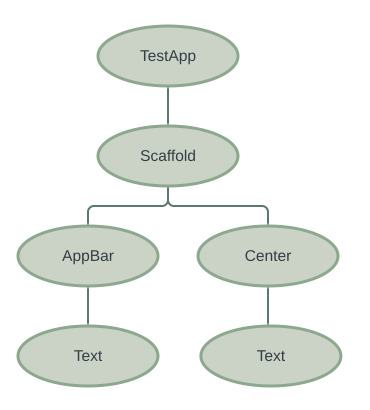
\includegraphics[scale=0.12]{stakeholder_matrix.png}
	\caption[Power/Interest Grid for Stakeholder-Analysis ]{Power/Interest Grid for Stakeholder-Analysis}
\end{figure}
\noindent	
Based on the classification of stakeholders in the matrix, the following statements can be made (based on \cite{.stakes}):
\newline \\
A close relationship should be maintained with the developer's personas and the application users. They should be allowed to give their feedback on the application, and their opinion should be considered in the development process.
\newline \\ 
Within the application doctors will also be users of the application and should be treated accordingly. However, since they cannot be categorized within the stakeholder matrix, as their impact on the project can be very different, special attention should be paid to them. This includes that they should always be satisfied so they do not bring bad words about the application to their patients. They should always be kept informed and monitored. Again, a close relationship should be maintained, and their opinion should be highly valued.

\section{System Context Diagram}
The greater environment in which a specific system or process functions is known as the system context. It covers all the outside variables and influences that affect the system's function, such as the stakeholders impacted by its operation, external systems and processes with which it interacts, and the policies and regulations it must comply with \cite{.systemcontext}. The system context can be determined using the previously performed stakeholder analysis. Determining the system context helps to understand which components interact with the system. This includes both the stakeholders and systems that influence the system.
\newline \\
The stakeholder groups of users and doctors can access the application via a smartphone. The developer and the database communicate with the system via direct code-based access. The database is filled with data from an API, and both impact the system. There are some aspects of the privacy policy and the security of the user's data, especially during the verification process of the doctors. Since, in the context of this bachelor thesis, the application will not be launched on the Play Store, these aspects are not addressed in the system context.

\begin{figure}[H]
	\centering
	\includegraphics[scale=0.13]{system_context.png}
	\caption[System Context Diagram ]{System Context Diagram}
\end{figure}

\section{User Requirements Specification}
The requirements for an application can be divided into three categories: functional requirements, non-functional requirements, and optional requirements \cite[p. 51 ff.]{.req2} \cite{.req}. In this section, the different requirements are considered and created project-specifically. An overview of all system requirements can be found in Appendix C.

\subsection{Optional Requirements}
As the name suggests, optional requirements of an application consist of requirements that do not necessarily have to be implemented. As seen from the first survey, which can be found in Appendix A, users would like to be able to save their diagnoses. This wish forms the optional requirement 1  \textbf{([OR1])}. Another optional requirement for the system could be that a user gets the ability to save advice they browse as well - similar to the collection feature on Instagram \textbf{([OR2])}. This allows him to quickly filter and retrieve his stored advice.

\subsection{Functional Requirements}
Functional requirements are the specific capabilities, behaviors, and features that a system must have. They describe how the system must work to succeed and provide a basis for evaluating its performance and functionality. First, it should be possible for the user to switch back and forth between the different views of the application \textbf{([FR1])}. Furthermore, users shall be able to verify themselves as a doctor \textbf{([FR2]} and subsequently log in as such \textbf{([FR3])}. Once this is done, these doctors must be provided with the functionality to add new records to the database \textbf{([FR4])} and also to modify existing records \textbf{([FR5])}. Based on these records, a user should be able to start a new diagnosis \textbf{([FR6])}, which he can also save \textbf{([FR7])} and view again \textbf{([FR8])}. If the user wants to cancel the diagnosis, the system must be able to allow him to do so at any time \textbf{([FR9])}. After a diagnosis has been successfully made and saved, it must also be possible to delete the diagnosis \textbf{([FR10])}. Likewise, it should be possible for a doctor to cancel the addition or modification of data records at any time \textbf{([FR11])}. 


\subsection{Non-functional Requirements}
After the functional requirements have been determined, the non-functional requirements are now considered. Non-functional requirements can be described as not dealing with a user's direct interaction with the application but with the system-specific properties. This includes, for example, the reliability of the application but also safety aspects \cite{.req2}. For example, a non-functional requirement for the system is that it should be able to make correct diagnoses \textbf{([NFR1])} and do so without requiring a user to log in \textbf{([NFR2])}. In addition, the graphical interface should be intuitive for the user \textbf{([NFR3])} to ensure user-friendliness.



\section{Use Cases}
The application's architectural goal is to provide an optimal user experience for patients and doctors. In order to ensure this, it is necessary to determine, before the actual development, which uses cases the software has to cover, i.e., the externally visible interactions of the users with the system. This ensures that the application meets the users' wishes and that they use it. In addition, possible ambiguities are revealed, and required data structures are determined. Possible problems that may arise during the application use are likely to be found during the process, and technical solutions can then be worked out. Experience has shown that use cases also make it easier for a developer to create the objects that have to be created with an object-oriented programming language in the early development process more precisely and to recognize and implement inheritance options at an early stage. Some use cases can be identified from the functional and optional requirements above. Figure 3.3 shows the resulting use case diagram, which has been shortened to the most relevant use cases. 

\begin{figure}[H]
	\centering
	\includegraphics[scale=0.175]{use_case_diagram.png}
	\caption[Use Case Diagram]{Use Case Diagram}
\end{figure}
\noindent
The use cases are described in detail in the following sections. The resulting use case tables for each of them can be found in Appendix D.

\subsection{Get Diagnosis}
The first use case is deprived by the fact that a user would like to receive a diagnosis \textbf{[FR6]}. The actors who can carry out this use case are both patients and doctors. In this application, doctors represent a subclass of users. In order to start the disease determination, the trigger, which will be implemented in the form of a button, must be pressed. The system then responds by displaying the view to enter and specify symptoms. As soon as the actor has finished specifying the symptoms, the system calculates the possible diseases and displays them to the actor as a diagnosis. The actor now has the opportunity to decide whether he wants to end the use case by exiting the diagnostic view or saving the diagnosis \textbf{[FR7]}, which is indicated by pressing the save button. The system then saves the diagnosis. Optionally, the actor should also be able to save the diagnosis as a PDF on his device \textbf{[OR1]}. During the process, the user can cancel the symptom statement at any time, which ends the use case by returning to the main page of the application \textbf{[FR10]}.

\subsection{Review Received Diagnoses}
After the user has received his diagnosis, he should be able to look at old diagnoses again \textbf{[FR8]}. The prerequisite for seeing such a diagnosis is that the actor had previously saved it when the diagnosis was made. A view is provided in the application in which saved diagnoses are displayed in a list. Clicking on such a diagnosis starts the use case, on which the system opens the detailed view of the diagnosis. The use case is ended by clicking on the back button provided for this purpose. While the diagnosis is being viewed, the user can delete the selected diagnosis. This is triggered by clicking on the icon provided for this purpose and is answered by deleting the diagnosis from the system. In this use case, the user is allowed to save his diagnosis as a PDF \textbf{[OR1]} too. The procedure for this corresponds to that of the "Get Diagnosis" use case.

\subsection{Login}
As mentioned in the project goal, doctors should be allowed to log into the application \textbf{[FR3]}. The trigger for the use case is the click on the login button. Once the button is pressed, the application will display the login page. The actor can enter his credentials, at which point the system checks whether these are stored in the database. Should the result be positive, the doctor will be logged in, and the system will display the doctor's dashboard. The prerequisite for the use case to be carried out without errors is that the doctor has been able to verify himself as such beforehand \textbf{[FR2]}. If this has not happened yet, the user can click on the verify button, where he will be prompted to carry out this process and will be logged in if it is successful. Should it be not successful because the user can not verify himself as a doctor, the system will continue showing error messages to the actor. Supposing the doctor is verified, but the system cannot find the entered credentials. Suspecting that the credentials have been entered incorrectly, the application displays an error message and the user is asked to check his user data and try again after correcting possible input errors.

\subsection{Add Data}
Provided that he is logged in, a doctor can now add data to the database \textbf{[FR4]}. In order to do this, he has to press the button provided for this purpose. The system then displays the blank template for a data record, in which the doctor can enter the data he wants to add. As soon as he has done this and pressed the confirm button, the system adds the data record to the database and saves it in his data list. Suppose the actor presses the confirm button without entering anything in each data field. In that case, the application will display an error notification on the screen, prompting the user to fill in all data fields. If the user wishes to cancel the process, he is free to press the button provided for this at any time, after which the system closes the view and the use case ends \textbf{[FR11]}. 

\subsection{Edit Data}
In addition to the functionality to create new datasets, the doctor should be able to expand and edit existing datasets \textbf{[FR5]}. The structure of this use case is similar to the previously described use case of adding new data. The doctor must first be in the view where all existing data records are displayed in list format. There he has the opportunity to click on one of these data sets, which signals to the system that it must now display the editing screen for the selected data set. In this view, the doctor can make the desired changes and press the confirm button. The application will then update the record in the database, and the use case will be terminated. As before, when adding new data records, the doctor can end the process at any time \textbf{[FR11]}.

\subsection{Get Tips and Tricks for Symptoms and Diseases}
The final use case worth mentioning is viewing advice on illnesses \textbf{[FR1]}. A user can go to the view for all advice that Doctors have uploaded. Once he has navigated there and the system shows the predicted view, he can click on one of the pieces of advice there, which will be shown to him in detail afterward. Optionally, the user can save the advice as a favorite by clicking on the button provided for this purpose \textbf{[OR2]}. 

\section{Domain Model}
Domain modeling is a vital modeling topic in Agile development at scale because there is frequently a gap between comprehending the issue domain and interpreting requirements. It depicts the solution as a collection of domain objects that collaborate to satisfy system-level scenarios \cite{.safe}. The quintessence of the object-oriented analysis step is decomposing a domain into problem-relevant concepts or objects. A domain model is a visual representation of the problem-relevant domain classes of a domain \cite{.safe}. With the help of unified modeling language (UML) notation, a domain model is represented by a set of class diagrams defined \cite{.domainmodel}. They usually consist of no methods or functions. It presents a conceptual perspective and can show domain objects or classes, as well as associations between domain classes and attributes of domain classes \cite{.safe} \cite{.domainmodel}. Identifying domain entities and their connections, derived from a grasp of system-level requirements, offers a good foundation for understanding and supports practitioners in designing systems for maintainability, testability, and incremental development \cite{.safe}. Finding conceptual classes by recognizing substantive phrases is an effective technique for domain modeling \cite[p. 76]{.domainmodel}.

\begin{itemize}
	\item A person is a \textbf{user} of the application.
	\item A \textbf{user} chooses a \textbf{body part}.
	\begin{itemize}
		\item A \textbf{body part} can be associated with different \textbf{symptoms}.
		\item A \textbf{user} selects a \textbf{symptom} and specifies the selected symptom by narrowing down (selecting) \textbf{proposed symptoms}, the \textbf{time of occurrence} and the \textbf{symptom intensity}. The information obtained is summarized as a textbf{user-specified symptom}.
	\end{itemize}
	\item One or more \textbf{user-specified symptoms} lead to the calculation of one or more possible \textbf{diseases}.
	\begin{itemize}
		\item A \textbf{disease} has different \textbf{symptoms}.
	\end{itemize}
	\item A \textbf{diagnosis} consists of one or more \textbf{diseases}.
	\item \textbf{Doctors} are special \textbf{users} of the application.
	\item \textbf{Doctors} can add/edit \textbf{advices}, \textbf{symptoms}, \textbf{body parts} and \textbf{diseases}.
	\item \textbf{Users} can view \textbf{advices}.  
\end{itemize}
\noindent
The information just obtained makes it easier to create the domain model. The entities user, symptom, user-specified symptom, body part, diseases, doctor, advice, and diagnosis, can already be recognized. Based on that information, a domain model can be created. 
\begin{figure}[H]
	\centering
	\includegraphics[scale=0.225]{domain_model.png}
	\caption[Domain Model]{Domain Model}
\end{figure}
\noindent
Based on the domain model and the previously obtained information, database development can now be started. Later on, the chapter optimizations also address some aspects that have been neglected.

 
  
  
\chapter{The Database}

\section{Introduction to NoSQL Datbases}
The term NoSQL describes database systems that, unlike SQL databases, are not subject to the relational database model. The abbreviation NoSQL stands for "Not only SQL". The reasons why NoSQL databases have gained interest in recent years can be explained on the basis of two aspects: In contrast to relational databases, which present their data storage in table format, NoSQL databases benefit from different database models: document-oriented, key Value, graph and column databases.[Image] This wide range of different data models gives developers the benefit of being able to choose the model that best suits their application design. The resulting result is a minimization of the code to be developed for an application. In addition, NoSQL databases allow administrators to scale their data both on one machine and on hardware clusters, so data volumes can be expanded without an expensive investment in new servers.
 \begin{figure}
	\centering
	\includegraphics[scale=0.3]{nosql.jpg}
	\caption[NoSQL Data Models]{NoSQL Data Models}
\end{figure}
\section{Firestore}
Cloud Firestore, more often called Google Firestore, is a cloud-hosted NoSQL database option which enables developers to store and synchronize their data in realtime, meaning that data which just got added to the database and changes made on already existing data are instantly shown to the application users. Since Firestore is published by Google, it comes with peak reliablitly and great performance.  Firestore can easily be integrated in a Flutter Application with help of public packages and via the native SDKs. Something worth to mention is, that Firestore can be used with far more programming languages than Dart and is also compatible with REST and RPC APIs. Cloud Firestore caches data that your app is actively using, so the app can write, read, listen to, and query data even if the device is offline. When the device comes back online, Cloud Firestore synchronizes any local changes back to Cloud Firestore. To keep your data safe, firestore offers the opportunity to create security rules based on an individuals needs, this includes Identy and Access Management (IAM).

With Firestore in combination with Flutter one can retrieve data via the package cloud\_firestore and the StreamBuilder Widget provided by Flutter. The named package also allows the developer to make use of the authentication functionality provided by firestore, which makes it possible for a user to register and login in an application. A detailed example will be given later on, when adding and retrieving data becomes relevant in the diagnose-tracker-application. 

\section{Document Databases}
As mentioned in the introduction to NoSQL databases, there are several different databases which all rely on different data models. Firestore makes use of the document-based data format. This means, that data stored in the database is accessible via collections, which are filled with documents. For better understanding one can imagine a collection in Firestore as a table in relational Databases and a Document in Firestore equals a row in the relational schema. An example of that is shown in the figure x.x. Documents in Firestore store their data in a key-value-format which makes it possible for a developer to store different sort of documents in each collection. A quick view at an example makes this easier to understand: A developer wants to develop a restaurent-review application. For that he creates a collection named “restaurants” in firestore. Two of the three restaurants he now wants to add to the collection got a slogan with their brand which he wants to add to the documents, the other restaurant doesn’t have one. In a relational database he still would have to fill the “slogan” column with at least NULL-data or an empty String (or whatever datatype the column has). Firestore, or document-based databases in general, allow it, to just not add the slogan attribute to the third restaurant, which helps to only store relevant data to the database. It is important to keep in mind, that even if the third restaurant one day gets a slogan, the developer has the possibility to add that field to the document later on. Cloud Firestore also allows it to store subcollections or complex nested objects to documents. When wanting to recieve data from Firestore, one can simply 

\section{Data Structure}
The data structure of the database is based on the decision that the ApiMedic API will be the main supplier of the data. The basic data structure can already be guessed from the domain model, which is shown in Figure 3.4. Firestore supports the following datatypes: String, Number, Boolean, Map, Array, Null, Timestamp, Geopoint and Reference. With a closer look at the API's JSON responses, the data structures can be formed.

\section{Firebase Redundancy}
\section{Inserting the Data into the Database}
JupyterNotebook - python code
\section{Connecting the Database with the Flutter Project}

  
  
%% PLANUNG %% 

\chapter{Development}

\section{Architecture: The Domain model (Flutter, Layered Architecture}
\section{Graphical User Interface}
\subsection{Survey}
\subsection{Design of the Graphical User Interface}
\subsection{Development of the Graphical User Interface}
\section{State Management of the Application}
\section{Symptomanalysis}
\section{Generate Diagnose PDF}
\section{Store PDF Locally on Device}
\section{Design Tip and Trick View}
\section{Doctor Login}
\section{Doctor Add/Edit Illnesses}
\section{Doctor Add/Edit Tips and Tricks}


  
  
%% PROOF OF CONCEPT %% 

\chapter{Development of the Match Algorithms}
\section{The Symptom Graph}
\section{Weighting of the Symptoms within the Application}
\section{Development of the Algorithms}
\section{Evaluation of the Algorithms}
\subsection{Performance Evaluation}
\subsection{Scalability Comparison}



  
  %
%% FAZIT %% 

\chapter{General Overview of the Application}
\section{Testing the Application}
\section{Survey: Would Respondents use this Application and put their trust in it}


  
  \include{kapitel/60_fazit}
  
  \include{kapitel/70_fazit}
  \begin{sloppypar}
  \printbibliography %Citavi 5
\end{sloppypar}
\end{document}